\documentclass[12pt]{beamer}
\usepackage{datetime}
\usepackage{tikz}
\usepackage{animate}
\usepackage{color}
\usetheme{Berlin}

\title[Employer Search and Screening in an Online Labor Market]{Employer Search and\\Screening in an Online\\Labor Market}
\author{John J. Horton}
\institute{oDesk Research}

\setbeamertemplate{footline}{%
  \begin{beamercolorbox}[sep=1mm,wd=\paperwidth,leftskip=1mm,rightskip=1mm]{footlinecolor}
    \hspace{1mm}%
    \tiny{\insertdate}
    \hfill
  \end{beamercolorbox}%
}

%gets rid of navigation symbols
\setbeamertemplate{navigation symbols}{}

%our items
\newcommand*\ouritem{%
\item[\color{black}\scalebox{0.9}{\textbullet}]}

%our imaginary items - that is, placeholders for items
\newcommand*\imgitem{%
\item[\color{white}\scalebox{0.9}{\textbullet}]}

\tikzstyle{every picture}+=[remember picture]
\tikzstyle{na} = [baseline=-.5ex]

\definecolor{myred}{RGB}{166,0,0}
\newcounter{boxes}

\newcommand\redbox[3]{%
\stepcounter{boxes}%
\begin{tikzpicture}[remember picture,overlay]
  \node[rectangle,rounded corners,line width=1pt,
      draw=myred,fill=myred!30,text height=20pt,
      text depth=11pt,align=left,fill opacity=0.7,text opacity=1] 
    (box-\theboxes) at #3 {#2};
  \node[rectangle,rounded corners,fill=myred!90,
      font={\Large\color{white}},anchor=west] 
    at ([xshift=10pt,]box-\theboxes.north west) {#1};
\end{tikzpicture}%
}

\newcommand\invbox[2]{%
\stepcounter{boxes}%
\begin{tikzpicture}[remember picture,overlay]
  \node 
    (box-\theboxes) at #2 {#1};
\end{tikzpicture}%
}

\begin{document}

\setlength{\baselineskip}{12mm}
\fontsize{10mm}{12mm}\selectfont

\begin{frame}
\begin{center}
Employer Search and\\
Screening in an Online\\
Labor Market

\vspace{3mm}

\large
John J. Horton\\
oDesk Research
\end{center}
\end{frame}

\begin{frame}{}
\begin{center}
Matching markets have

search screening costs
\end{center}
\end{frame}

\begin{frame}{}
\begin{animateinline}[autoplay]{2}
\begin{minipage}{\textwidth}
\Large
\begin{itemize}
\imgitem \textcolor{white}{What \emph{are} my options?}

\imgitem \textcolor{white}{\emph{How good} is each option for me?}
\end{itemize}
\end{minipage}
\newframe
\begin{minipage}{\textwidth}
\Large
\begin{itemize}
\ouritem What \emph{are} my options?

\imgitem \textcolor{white}{\emph{How good} is each option for me?}
\end{itemize}
\end{minipage}
\newframe
\begin{minipage}{\textwidth}
\Large
\begin{itemize}
\ouritem What \emph{are} my options?

\ouritem \emph{How good} is each option for me?
\end{itemize}
\end{minipage}
\end{animateinline}
\end{frame}

\begin{frame}{}
\begin{animateinline}[autoplay]{2}
\begin{minipage}[c]{1\textwidth}
\begin{center}
\Large

\begin{figure}[H] \centering 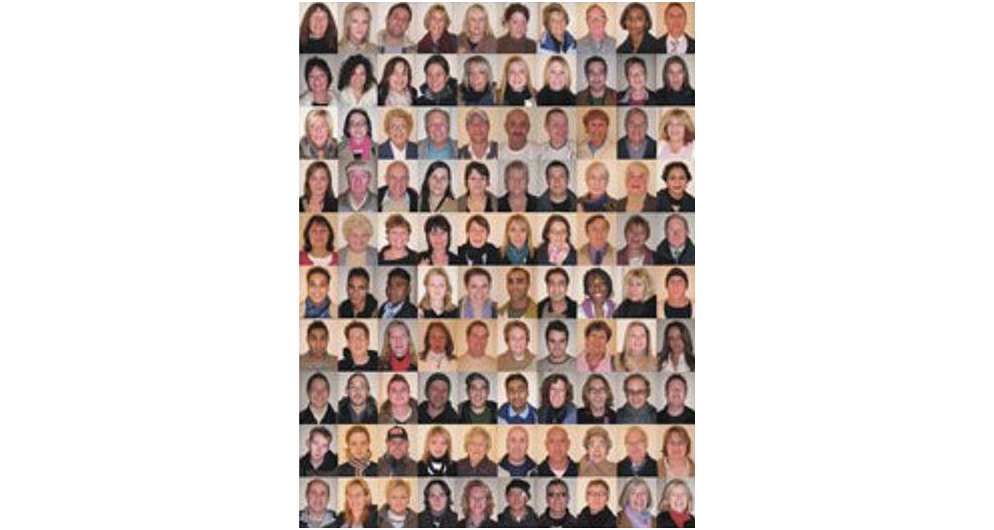
\includegraphics[width=100mm]{people_animation_1.png} \end{figure}

100 people
\end{center}
\end{minipage}
\end{animateinline}
\end{frame}

\begin{frame}{}
\begin{animateinline}[autoplay]{10}
\multiframe{11}{i=1+1}{
\begin{minipage}[c]{1\textwidth}
\begin{center}
\Large

\begin{figure}[H] \centering \includegraphics[width=100mm]{people_animation_\i.png} \end{figure}

100 people
\end{center}
\end{minipage}
}
\newframe
\multiframe{9}{i=11+1}{
\begin{minipage}[c]{1\textwidth}
\begin{center}
\Large

\begin{figure}[H] \centering \includegraphics[width=100mm]{people_animation_\i.png} \end{figure}

1,000 people
\end{center}
\end{minipage}
}
\end{animateinline}
\end{frame}

\begin{frame}{}
\begin{animateinline}[autoplay]{10}
\multiframe{5}{i=1+1}{
\begin{minipage}[c]{1\textwidth}
\begin{center}
\Large

\begin{figure}[H] \centering \includegraphics[width=100mm]{people_animation_2_\i.png} \end{figure}

1,000 people
\end{center}
\end{minipage}
}
\newframe
\multiframe{6}{i=6+1}{
\begin{minipage}[c]{1\textwidth}
\begin{center}
\Large

\begin{figure}[H] \centering \includegraphics[width=100mm]{people_animation_2_\i.png} \end{figure}

100,000 people
\end{center}
\end{minipage}
}
\end{animateinline}
\end{frame}

\begin{frame}{}
\begin{animateinline}[autoplay]{10}
\multiframe{10}{i=1+1}{
\begin{minipage}[c]{1\textwidth}
\begin{center}
\Large

\begin{figure}[H] \centering \includegraphics[width=100mm]{people_animation_3_\i.png} \end{figure}

100,000 people
\end{center}
\end{minipage}
}
\newframe
\multiframe{8}{i=11+1}{
\begin{minipage}[c]{1\textwidth}
\begin{center}
\Large

\begin{figure}[H] \centering \includegraphics[width=100mm]{people_animation_3_\i.png} \end{figure}

1,000,000 people
\end{center}
\end{minipage}
}
\end{animateinline}
\end{frame}

\begin{frame}{}
\begin{center}
Algorithmic approach
\end{center}

\begin{animateinline}[autoplay]{2}
\begin{minipage}{\textwidth}
\Large
\begin{itemize}
\imgitem \textcolor{white}{Infer nature of the work}

\imgitem \textcolor{white}{Find candidates with matching skills}

\imgitem \textcolor{white}{Sort matching candidates by some weighted combination of ability \& availability}
\end{itemize}
\end{minipage}
\newframe
\begin{minipage}{\textwidth}
\Large
\begin{itemize}
\ouritem Infer nature of the work

\imgitem \textcolor{white}{Find candidates with matching skills}

\imgitem \textcolor{white}{Sort matching candidates by some weighted combination of ability \& availability}
\end{itemize}
\end{minipage}
\newframe
\begin{minipage}{\textwidth}
\Large
\begin{itemize}
\ouritem Infer nature of the work

\ouritem Find candidates with matching skills

\imgitem \textcolor{white}{Sort matching candidates by some weighted combination of ability \& availability}
\end{itemize}
\end{minipage}
\newframe
\begin{minipage}{\textwidth}
\Large
\begin{itemize}
\ouritem Infer nature of the work

\ouritem Find candidates with matching skills

\ouritem Sort matching candidates by some weighted combination of ability \& availability
\end{itemize}
\end{minipage}
\end{animateinline}
\end{frame}

\begin{frame}{}
\begin{center}
What segments matching

markets traditionally?
\end{center}

\begin{animateinline}[autoplay]{2}
\begin{minipage}{\textwidth}
\Large
\vspace{1 mm}
\begin{itemize}
\imgitem \textcolor{white}{Geography}

\imgitem \textcolor{white}{Time}

\imgitem \textcolor{white}{Costs of application}
\end{itemize}

\nointerlineskip
\begin{tikzpicture}[overlay]
\end{tikzpicture}
\end{minipage}
\newframe
\begin{minipage}{\textwidth}
\Large
\vspace{1 mm}
\begin{itemize}
\ouritem Geography

\imgitem \textcolor{white}{Time}

\imgitem \textcolor{white}{Costs of application}
\end{itemize}

\nointerlineskip
\begin{tikzpicture}[overlay]
\end{tikzpicture}
\end{minipage}
\newframe
\begin{minipage}{\textwidth}
\Large
\vspace{1 mm}
\begin{itemize}
\ouritem Geography

\ouritem Time

\imgitem \textcolor{white}{Costs of application}
\end{itemize}

\nointerlineskip
\begin{tikzpicture}[overlay]
\end{tikzpicture}
\end{minipage}
\newframe
\begin{minipage}{\textwidth}
\Large
\vspace{1 mm}
\begin{itemize}
\ouritem Geography

\ouritem Time

\ouritem Costs of application
\end{itemize}

\nointerlineskip
\begin{tikzpicture}[overlay]
\end{tikzpicture}
\end{minipage}
\newframe[20]
\begin{minipage}{\textwidth}
\Large
\vspace{1 mm}

\begin{itemize}
\ouritem \tikz[na] \node[coordinate] (geo1) {};G\tikz[na] \node[coordinate] (geo2) {};eography

\ouritem Time

\ouritem Costs of application
\end{itemize}

\nointerlineskip
\begin{tikzpicture}[overlay]
\draw[line width=2pt,red] (geo1) edge [out=0, in=180] (geo2);
\end{tikzpicture}
\end{minipage}
\newframe
\begin{minipage}{\textwidth}
\Large
\vspace{1 mm}

\begin{itemize}
\ouritem \tikz[na] \node[coordinate] (geo1) {};Ge\tikz[na] \node[coordinate] (geo2) {};ography

\ouritem Time

\ouritem Costs of application
\end{itemize}

\nointerlineskip
\begin{tikzpicture}[overlay]
\draw[line width=2pt,red] (geo1) edge [out=0, in=180] (geo2);
\end{tikzpicture}
\end{minipage}
\newframe
\begin{minipage}{\textwidth}
\Large
\vspace{1 mm}

\begin{itemize}
\ouritem \tikz[na] \node[coordinate] (geo1) {};Geo\tikz[na] \node[coordinate] (geo2) {};graphy

\ouritem Time

\ouritem Costs of application
\end{itemize}

\nointerlineskip
\begin{tikzpicture}[overlay]
\draw[line width=2pt,red] (geo1) edge [out=0, in=180] (geo2);
\end{tikzpicture}
\end{minipage}
\newframe
\begin{minipage}{\textwidth}
\Large
\vspace{1 mm}

\begin{itemize}
\ouritem \tikz[na] \node[coordinate] (geo1) {};Geog\tikz[na] \node[coordinate] (geo2) {};raphy

\ouritem Time

\ouritem Costs of application
\end{itemize}

\nointerlineskip
\begin{tikzpicture}[overlay]
\draw[line width=2pt,red] (geo1) edge [out=0, in=180] (geo2);
\end{tikzpicture}
\end{minipage}
\newframe
\begin{minipage}{\textwidth}
\Large
\vspace{1 mm}

\begin{itemize}
\ouritem \tikz[na] \node[coordinate] (geo1) {};Geogr\tikz[na] \node[coordinate] (geo2) {};aphy

\ouritem Time

\ouritem Costs of application
\end{itemize}

\nointerlineskip
\begin{tikzpicture}[overlay]
\draw[line width=2pt,red] (geo1) edge [out=0, in=180] (geo2);
\end{tikzpicture}
\end{minipage}
\newframe
\begin{minipage}{\textwidth}
\Large
\vspace{1 mm}

\begin{itemize}
\ouritem \tikz[na] \node[coordinate] (geo1) {};Geogra\tikz[na] \node[coordinate] (geo2) {};phy

\ouritem Time

\ouritem Costs of application
\end{itemize}

\nointerlineskip
\begin{tikzpicture}[overlay]
\draw[line width=2pt,red] (geo1) edge [out=0, in=180] (geo2);
\end{tikzpicture}
\end{minipage}
\newframe
\begin{minipage}{\textwidth}
\Large
\vspace{1 mm}

\begin{itemize}
\ouritem \tikz[na] \node[coordinate] (geo1) {};Geograp\tikz[na] \node[coordinate] (geo2) {};hy

\ouritem Time

\ouritem Costs of application
\end{itemize}

\nointerlineskip
\begin{tikzpicture}[overlay]
\draw[line width=2pt,red] (geo1) edge [out=0, in=180] (geo2);
\end{tikzpicture}
\end{minipage}
\newframe
\begin{minipage}{\textwidth}
\Large
\vspace{1 mm}

\begin{itemize}
\ouritem \tikz[na] \node[coordinate] (geo1) {};Geograph\tikz[na] \node[coordinate] (geo2) {};y

\ouritem Time

\ouritem Costs of application
\end{itemize}

\nointerlineskip
\begin{tikzpicture}[overlay]
\draw[line width=2pt,red] (geo1) edge [out=0, in=180] (geo2);
\end{tikzpicture}
\end{minipage}
\newframe
\begin{minipage}{\textwidth}
\Large
\vspace{1 mm}

\begin{itemize}
\ouritem \tikz[na] \node[coordinate] (geo1) {};Geography\tikz[na] \node[coordinate] (geo2) {};

\ouritem Time

\ouritem Costs of application
\end{itemize}

\nointerlineskip
\begin{tikzpicture}[overlay]
\draw[line width=2pt,red] (geo1) edge [out=0, in=180] (geo2);
\end{tikzpicture}
\end{minipage}
\newframe
\begin{minipage}{\textwidth}
\Large
\vspace{1 mm}

\begin{itemize}
\ouritem \tikz[na] \node[coordinate] (geo1) {};Geography\tikz[na] \node[coordinate] (geo2) {}; 
\invbox{
\small
\textcolor{red}{No inherent geographic constraints}}{(0.3\textwidth,0.025\textheight)}
\invbox{
\small
\textcolor{red}{in online labor markets}}{(0.3\textwidth,-0.025\textheight)}

\ouritem Time

\ouritem Costs of application
\end{itemize}

\nointerlineskip
\begin{tikzpicture}[overlay]
\draw[line width=2pt,red] (geo1) edge [out=0, in=180] (geo2);
\end{tikzpicture}
\end{minipage}
\end{animateinline}
\end{frame}

\end{document}